\section{Preprocessing}
\tikzstyle{diabox}=[minimum height=1.4cm,shape=rectangle,align=center, draw, font=\small]
\begin{figure*}[t]
    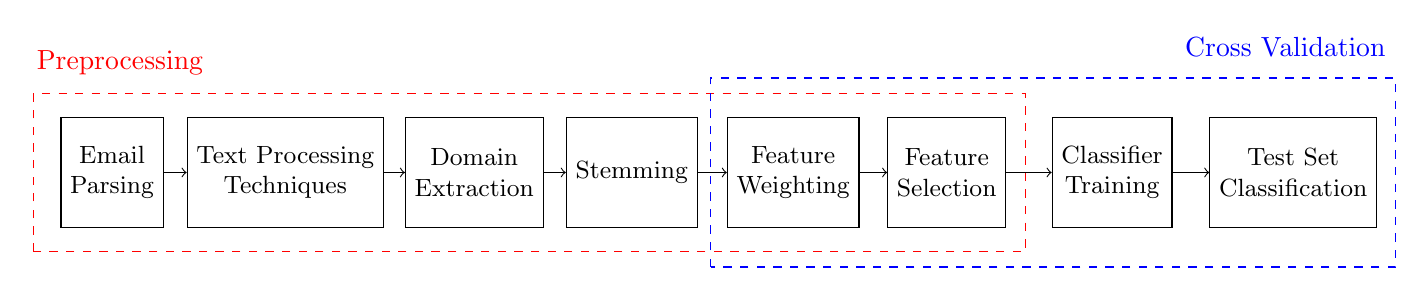
\begin{tikzpicture}
        \node[diabox] at (0.00,0) (parsing) {Email\\Parsing};
        \node[diabox] at (2.2,0,0) (textproc) {Text Processing\\Techniques};
        \node[diabox] at (4.6,0) (domain) {Domain\\Extraction};
        \node[diabox] at (6.6,0) (stemming) {Stemming};
        \node[diabox] at (8.65, 0) (weight) {Feature\\Weighting};
        \node[diabox] at (10.6,0)  (fselection) {Feature\\Selection};
        \node[diabox] at (12.7, 0) (training) {Classifier\\Training};
        \node[diabox] at (15, 0) (classify) {Test Set\\Classification};
        \draw[red,dashed] (-1,-1) rectangle ++(12.6,2);
        \draw[red] (0.1,1.4) node {Preprocessing};
        \draw[blue,dashed] (7.6,-1.2) rectangle ++(8.7,2.4);
        \draw[blue] (14.9,1.6) node {Cross Validation};
        \draw [->] (parsing.east) -- (textproc.west);
        \draw [->] (textproc.east) -- (domain.west);
        \draw [->] (domain.east) -- (stemming.west);
        \draw [->] (stemming.east) -- (weight.west);
        \draw [->] (weight.east) -- (fselection.west);
        \draw [->] (fselection.east) -- (training.west);
        \draw [->] (training.east) -- (classify.west);
    \end{tikzpicture}
    \caption{Steps taken during training and cross validation}
    \label{fig:steps}
\end{figure*}

The bag of words model used by our classifiers is a good way to represent the data found in the given training documents. However this feature representation is prone to very high dimensions if not handled well due to the large number of possible combinations in words. 

According to a recent survey performed by Google and Harvard, there are approximately 1,022,000 different words in the English language \cite{google2010words}. While we do not expect to find all possible words in the document corpus, a large number of them will be found along with their derivations in the form of spelling mistakes and grammatical variations (e.g.{\it they're} and {\it theyre}). Other non-English words such as html code, URLs and nonsensical data such as PGP keys will also be found within the documents.

Most of these words will provide no benefit to the classifier and in most cases will even harm the classifier's performance. It is therefore of utmost importance that noise in the text is filtered out and the number of word combinations is reduced to the most representative, yet minimal subset of the available words. Once this is done, steps can be taken to transform each document into a feature vector that can be understood by the classifier. 

The following steps are taken to do this:
\begin{itemize}
	\item Smart Email Parsing
	\item Simple Text Processing Techniques
	\item Domain Extraction
	\item Stemming
	\item Inverted Index Storage
	\item Feature Selection based on Document Frequency
	\item Vector Generation / Feature Weighting
\end{itemize}

Each of these steps contribute towards achieving a higher accuracy and performance in the classifier and will be described in detail in the sections below.

\subsection{Email Parsing}
As a first preprocessing step, we modify the parsing of the email structure.
The provided emails sometimes contain metadata which is very redundant w.r.t. to the number of contained words, e.g. all will have a "From" line but also if an email has metadata is independent from its class label, i.e. the classifier should not that all mails that have metadata are spam.
Furthermore mails do not always consist of just text but also have attachments or their textual content is supplied as plain text or beautified with HTML markup.

In a first step, we strip the metadata from the email so that only give the content of the mail to the classifier.
This reduces the size of data passed on to the classifier as most terms in the metadata are either common among all emails, e.g. the names of the header lines (``From'', ``Content-Type'', \dots), or are unique to the mail like the date of sending or the message-id.
From the metadata we extract some basic information like the encoding or if it is a multi-part email for further processing.

If the mail is split in multiple parts, we want to extract only the parts which contain text as we cannot infer information of the \emph{base64} representation of images or other binary attachments.
These binary attachments would only add a large number of words of a length of 76 characters \cite{rfc2045} to the index which are very uncommon in other mails as images are compressed data with a high entropy.
Another problem that is solved by adding handling multiple is the recursive parsing of attached emails that have textual content and may have multiple parts again inside so that we are now stripping down the inner mails to their actual content too.

Furthermore not all text is encoded in the same encoding as the email itself, e.g. the main text could be encoded as Base64 which would not reveal the actual words when just splitting the mail into words by separating at each space.
Another typical encoding is quoted-printable which only transforms non-ASCII characters into another format but leaves all ASCII characters intact.
Handling these encoding turns meaningless, long character sequences into words that are present in other mails.

As a final parsing step in the email handling we are stripping all HTML from the mails to remove all HTML tags from our word index.
This markup is not displayed to the user and does not carry any content that will be some sort of advertising.

Although email parsing did not make a significant impact on the quality score of the classifier, it reduced its dimensionality from 143820 down to 94903.
With this lower dimensionality the runtime decreases too from 16 minutes to ten.
In conclusion email parsing stripped a lot of irrelevant or redundant dependencies from the input data set without the cost of quality loss.

\subsection{Simple Text Processing Techniques}

A number of simple processing techniques are used to conflate incoming strings that represent the word together. Although the email parser is built in such a way as to strip out html content where possible, a number of artefacts could still linger in the data which could cause noise and incorrectly distinguish variations of the same word. Because it is not the parsers job to perform this form of filtering, a separate step is taken to perform simple text processing tasks before passing them on the later pre-processing stages.

All incoming words that are composed purely of symbols (i.e. no numbers or letters) are simply discarded as they are most commonly noise in the data that does not represent anything in the corpus. Without this step, the number of features used by the classifier would grow substantially as a large number of "rubbish" symbols are included as part of the feature set. Additionally, all remaining words will have ally symbols stripped, this prevents variations in words like {\it they're} and {\it theyre} from being treated as different features.

As a second step, all valid incoming words are simply reduced to lower-case format. The same word in different cases should not be distinguished from one another during classification so it is important that e.g. {\it Bristol} is considered the same as {\it bristol}.

Finally, variations in number representations (e.g. 4,000 and 4000) are detected using regular expressions and conflated to a single representative feature "9999". We do this because allowing all possible number combinations each a unique feature will increase the dimensionality substantially and rarely contribute to classification performance - it can most often be considered noise. Doing this also provides some assurance that we do not overfit our classifier to the training set with specific numeric combinations.

Using the techniques described above we were able to reduce the number of  combinations from 94,903 words to just 56149. This provides a substantial decrease in dimensions and provides a very notable improvement to memory usage, training speed and classification speed. 

\subsection{Domain Extraction}

Due to the fact that Emails are a product of the web, it is very common to find items such as Uniform Resource Locaters (URLs) and email addresses within the their text. When left unprocessed, it is hard to group these items into corresponding features due to the additional data included within them.

What we really care about is the domain each URL and email address contains. If we find two URLs which point to the same domain such as \emph{www.cs.bris.ac.uk/maths} and {\it www.cs.bris.ac.uk/eng}, the it would make sense to group these two items together as one feature - i.e. coming from the domain \emph{cs.bris.ac.uk}. This will prove useful in being able to identify URLs which point to malicious or spam websites and those which are well known and credible domains.

To do this, we use a regular expression parser to detect items that are URLs and email addresses. Detected items are put through a \emph{Domain Extraction} function which is able to strip out the username and '@' symbol in the case of emails (e.g. \emph{johndoe@example.com} would become \emph{example.com}) and remove paths and protocol declerations in the case of URLs (e.g. \emph{https://www.example.com/myimage.jpg} would become \emph{example.com} once again). Conflating both email address domains and web URL domains makes sense because they represent the same source of information.


\subsection{Stemming}
Most words in the English language are derived from a \emph{morphological root} word that contains no prefixes or suffixes and conveys a very similar meaning to its derivation. A simple example of this is \emph{subscriber} and \emph{subscription} with their morphological root \emph{subscribe}. 

If we can reduce all incoming words into their root form, we would be able to substantially reduce the number of dimensions for our model while also ensuring that words representing the same underlying feature are stored under the same value.

Unfortunately, such a task is quite hard and would probably require the creation of a very large lookup table for each word in the English language along with its root. This is due to the fact that the English language is not a formal language and hence does not follow a strict set of rules. 

We could however, take an approximation of the described process and instead derive the \emph{stem} of each word. Like the morphological root, the stem is a representation of a words underlying meaning. However the stem does not guarantee to be a correct English word or generate the right root as its aim is simply to map variations of the same word to the same to item. 

For our Spam Filter implementation, we made use of the Porter Stemmer algorithm \cite{porter1980}, which in the authors words is ``a process for removing the commoner morphological and inflexional endings from words in English''. In simpler terms, it is capable of removing known suffixes from words passed to it. The Porter Stemmer algorithm is available as open source code under the BSD License and is available in multiple languages, including Java which is made use of in our implementation.

Using the same examples shown before, passing \emph{subscriber} and \emph{subscribe} to the Porter Stemmer would reduce the words \emph{subscribe} and \emph{subscriber} to the stem \emph{subscrib}. On the other hand, the word \emph{subscription} will be wrongly mapped to a different stem - \emph{subscript}. The latter is an example of where the approximation fails to produce the correct result, however in general most words passed to the algorithm have shown to produce favourable results.

In terms of the Spam Filter implementation, using Porter Stemming on the given set of training emails reduced the number of words from 24813 words to 18932 stems (both after text pre-processing). This is a substantial reduction in the number of dimensions and plays a crucial role in ensuring that the classifier is able to train with the given documents in a short amount of time and without requiring large amounts of memory. Apart from improving speed and reducing memory, it has also proved to improve classification performance.

\subsection{Inverted Index Storage}

After words have gone through simple text processing, domain extraction and stemming - they are stored in a fast inverted index structure in the form of a Hashed List. Using an inverted index allows quick querying of each term's metadata; such as its total frequency in the corpus and its frequency in each document. This information is especially important for the next two stages that will occur - Feature Selection and Feature Weighting.

\subsection{Feature selection}
Although we have substantially reduced the number of features through the use of various text processing techniques, we still have a substantial number of features for the classifier to train with. Interestingly, the frequency of occurrence for each word in the text can be grouped into 3 categories of very common, common and rare. 

Very frequent elements in the text and commonly referred to as stopwords in linguistic morphology. These are words which are very frequently found in English texts (Some good examples are \emph{the}, \emph{and}, \emph{it} etc..) and usually do not provide any particular indication about the category of the document's class. On the other hand, very rare elements in a text are usually attributed to spelling mistakes and other artefacts such as IDs (PGP keys being the most common in emails). In between these two categories we have words not too commonly found, but not rare enough to constitute as errors either.

A corpus of documents that shows this pattern is said to obey \emph{Zipf's law} \cite{zipf1949} and thus follow what is called a \emph{Zipfian Distribution}. It so happens that most English documents follow this law and so does our corpus. This is mainly due to a phenomenon pointed out by Zipf in his paper which he calls  \emph{the principle of least effort}.

The frequency of occurrence of each term in the given training set is shown in Figure \ref{zipfian}  mapped in descending order. Some words on the graph are specified on the x-axis to provide an example at each portion of the graph (Note that these are stems due to our previous Stemming technique). It should be immediately noted how common rare words are by the long "tail" shown in the graph and one should also notice how frequent certain words such as \emph{the} are.

What we really want to keep is the words which are in between these two categories as these are the most representative of the text. This area can be considered somewhat of a "\emph{Goldilocks Zone}" as its just about right for giving us the right information. To extract this area and remove the excess, we use a technique called feature selection to trim out all features from the index with a document frequency less than \(\alpha \times no. documents\)and more than \(\beta \times no. documents\), where \(\alpha\) and \(\beta\) are values in the range [0,1].

\begin{figure}[h!]
	\label{zipfian}
    \centering
    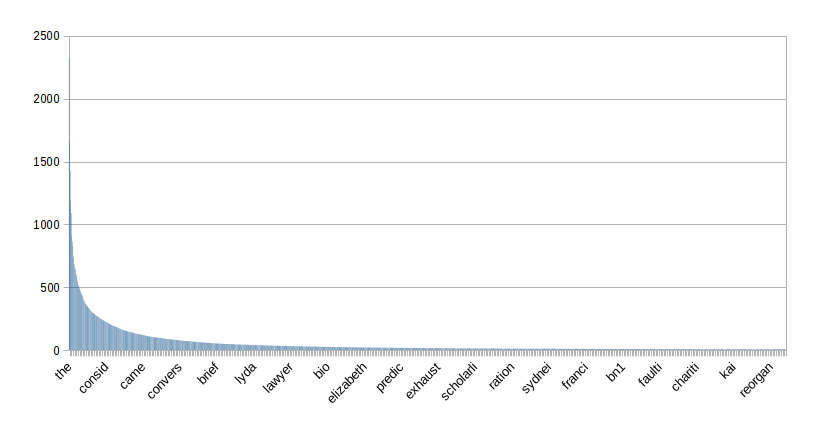
\includegraphics[width=0.5\textwidth]{zipfian.png}
    \caption{Zipfian Distribution exhibited in the Training Corpus}
    \label{zipfian}
\end{figure}

Unfortunately, choosing ideal \(\alpha \) and \(\beta\) is a somewhat tedious process of trial and error.
Finding the right values ensure that the classifiers does not overfit on features are only available in the training process but may accidentially strip out features that contribute very good to distinguish both classes but are represented with the same frequency as term that are considered irrelevant.
In Section \ref{sec:featurethresholds}, we will try to optimise our selected thresholds by the emperical evaluation of the performance of the classifier on out data set.

\subsection{Vector Generation / Feature Weighting}

Now that we have filtered out all unnecessary features and determined which features should be kept for classification, we need to convert email documents into data that is understandable by the Classifier. More specifically, we need to convert each email into a corresponding feature vector using the features we have just identified. In this report, we have attempted two ways of converting frequency information found in emails into corresponding weights. 

The first and most basic attempt uses \emph{Frequency Weighting} which is simply assigning each feature in a vector the frequency of the corresponding term in the email. 

The second approach taken is using \emph{Term Frequency Inverse Document Frequency} also commonly known as \emph{tfidf} \cite{tfidf1973}. Tfidf is a commonly used metric in natural language processing that portrays the importance of a word in a document with respect to the rest of the corpus. It is technique often used by Search Engines and has proven many times to be a reliable way of representing the significance of a term within a document. The equation for calculating the weight for a term $i$ in a document $j$ is given as:

\begin{align*}
	\textrm{tfidf}_{ij} = \frac{f_{ij}}{\textrm{maxf}} * \log\left(\frac{N}{n_i}\right)
\end{align*}

Where $N$ represents the number of documents, $n_i$ represents the number of times the term i appears in a document and \emph{maxf} represents the highest frequency in the document corpus.

After testing these two approaches, it was immediately noted that \emph{tfidf} gave significantly worse results than \emph{frequency weighting}. While this was initially a surprise, It was noted that this behaviour could be occurring due to use of a multinomial Naive Bayes model rather than Bernoulli model. \todo{maybe some more justification on this. Not sure this is enough information to justify mentioning tfidf}. We shall assume the use of Frequency Weighting for the rest of the report for this reason.

\subsection{Optimising Feature Thresholds}
\label{sec:featurethresholds}

After all preprocessing steps the total number of dimensions is now down to 43437 different words.
Altough this is less than a third of the initial dimensionality, it is slowing down the training of the classifier as well as the classification of the samples.
A high number of features can have a negative impact on quality of the classification results too as the classifier may learn to concentrate on words that are rare and only appear in the training set while leaving out feature that could separate the two classes very well.

To increase the quality and the runtime, we want to remove infrequent and non-separating, but still freuqent features without having a negative effect on the quality.
As an exhaustive search of all possible feature combination is infeasible, we will try to find emperically the two thresholds $\alpha$ and $\beta$.
This is done by setting one of the threasholds to a fixed value while iterating over possible values for the other threshold.

\begin{figure}[h!]
    \centering
    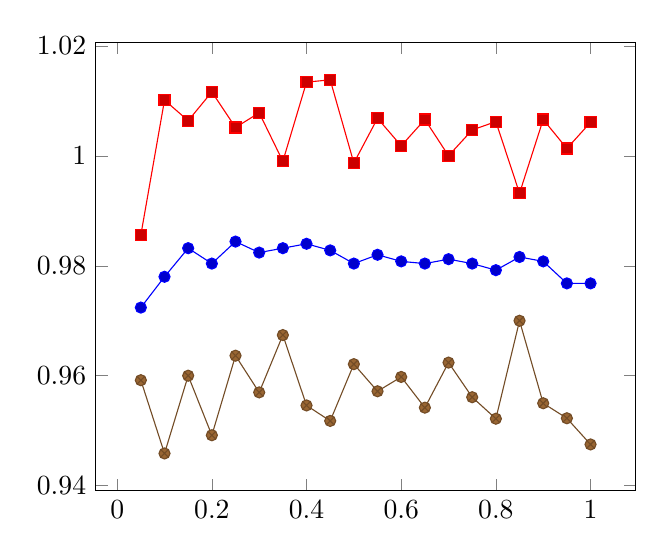
\begin{tikzpicture}
        \begin{axis}
             \addplot+[sharp plot] coordinates {
                (0.05, 0.972400)
                (0.10, 0.978000)
                (0.15, 0.983200)
                (0.20, 0.980400)
                (0.25, 0.984400)
                (0.30, 0.982400)
                (0.35, 0.983200)
                (0.40, 0.984000)
                (0.45, 0.982800)
                (0.50, 0.980400)
                (0.55, 0.982000)
                (0.60, 0.980800)
                (0.65, 0.980400)
                (0.70, 0.981200)
                (0.75, 0.980400)
                (0.80, 0.979200)
                (0.85, 0.981600)
                (0.90, 0.980800)
                (0.95, 0.976800)
                (1.00, 0.976800)
                };
             \addplot+[sharp plot] coordinates {
                (0.05, 0.972400+0.013206)
                (0.10, 0.978000+0.032125)
                (0.15, 0.983200+0.023186)
                (0.20, 0.980400+0.031215)
                (0.25, 0.984400+0.020746)
                (0.30, 0.982400+0.025424)
                (0.35, 0.983200+0.015799)
                (0.40, 0.984000+0.029394)
                (0.45, 0.982800+0.031010)
                (0.50, 0.980400+0.018287)
                (0.55, 0.982000+0.024819)
                (0.60, 0.980800+0.021014)
                (0.65, 0.980400+0.026199)
                (0.70, 0.981200+0.018804)
                (0.75, 0.980400+0.024298)
                (0.80, 0.979200+0.027011)
                (0.85, 0.981600+0.011593)
                (0.90, 0.980800+0.025799)
                (0.95, 0.976800+0.024528)
                (1.00, 0.976800+0.029285)
                };
             \addplot+[sharp plot] coordinates {
                (0.05, 0.972400-0.013206)
                (0.10, 0.978000-0.032125)
                (0.15, 0.983200-0.023186)
                (0.20, 0.980400-0.031215)
                (0.25, 0.984400-0.020746)
                (0.30, 0.982400-0.025424)
                (0.35, 0.983200-0.015799)
                (0.40, 0.984000-0.029394)
                (0.45, 0.982800-0.031010)
                (0.50, 0.980400-0.018287)
                (0.55, 0.982000-0.024819)
                (0.60, 0.980800-0.021014)
                (0.65, 0.980400-0.026199)
                (0.70, 0.981200-0.018804)
                (0.75, 0.980400-0.024298)
                (0.80, 0.979200-0.027011)
                (0.85, 0.981600-0.011593)
                (0.90, 0.980800-0.025799)
                (0.95, 0.976800-0.024528)
                (1.00, 0.976800-0.029285)
                };
    \end{axis}
    \end{tikzpicture}
    \caption{Accuracy w.r.t. upper threshold (lower threshold = 0)}
    \label{p:upperbound}
\end{figure}



To compare the impact on the behaviour of the classification of both classes \emph{Spam} and \emph{Ham} we are using the measures \emph{Precision}, \emph{Recall} and \emph{Negative Recall} as they are less dependent of the class distribution in the test set than \emph{Accuracy}.

In Figure \ref{p:upperbound}, we have set $\alpha = 0$ to have all lower frequent words in the training and iterating over $\beta$ to emperically determine which high frequent words can be removed without an effect on the cluster quality.
As seen in the graph, only for a value of $\beta$ larger than 0.19 all three quality measures stay quite constant.
In the interval between $0.05$ and $0.2$ there is a high variance of the scores, so we increased the resolution in the plot to a simulation in each 0.01 step to better view the behaviour of the classifier.
As a final choice for $\beta$ we have taken $\beta = 0.19$ as \emph{Recall} has its maximum here and decreases steep towards $\beta = 0$.
The other measures are at a very good level (near their maximum) for $\beta = 0.19$ and only increase slightly in this neighbourhood.

\begin{figure}[h!]
    \centering
    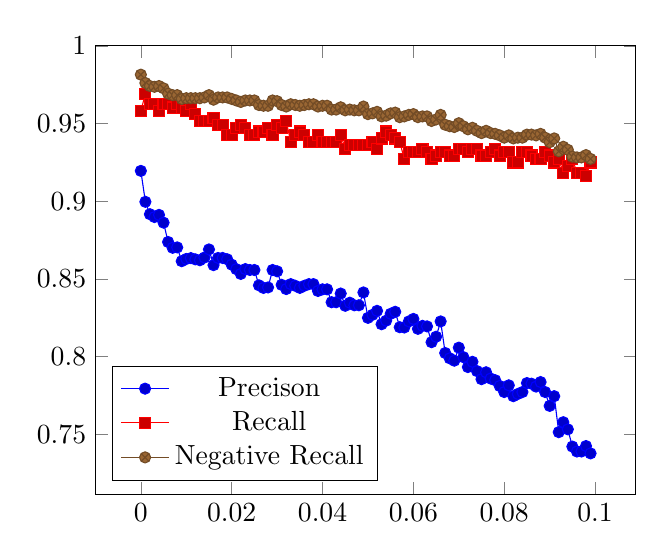
\begin{tikzpicture}
        \begin{axis}[
                legend pos=south west,
                ymax=1,
                xtick={0, 0.02, 0.04, 0.06, 0.08, 0.1},
                xticklabels={0, 0.02, 0.04, 0.06, 0.08, 0.1}
                ]
                \addplot+[sharp plot] coordinates {
                    (0.0, 0.919492)
                    (0.001, 0.899590)
                    (0.002, 0.891616)
                    (0.003, 0.889796)
                    (0.004, 0.891170)
                    (0.005, 0.886179)
                    (0.006, 0.873747)
                    (0.007, 0.870000)
                    (0.008, 0.870259)
                    (0.009, 0.861386)
                    (0.010, 0.862823)
                    (0.011, 0.863366)
                    (0.012, 0.862550)
                    (0.013, 0.862000)
                    (0.014, 0.863727)
                    (0.015, 0.868952)
                    (0.016, 0.858847)
                    (0.017, 0.863454)
                    (0.018, 0.863454)
                    (0.019, 0.862626)
                    (0.020, 0.859155)
                    (0.021, 0.856287)
                    (0.022, 0.853175)
                    (0.023, 0.856287)
                    (0.024, 0.855711)
                    (0.025, 0.855711)
                    (0.026, 0.845850)
                    (0.027, 0.844181)
                    (0.028, 0.844488)
                    (0.029, 0.855711)
                    (0.030, 0.854871)
                    (0.031, 0.846154)
                    (0.032, 0.843444)
                    (0.033, 0.846614)
                    (0.034, 0.845545)
                    (0.035, 0.844181)
                    (0.036, 0.845545)
                    (0.037, 0.846614)
                    (0.038, 0.846614)
                    (0.039, 0.842209)
                    (0.040, 0.843254)
                    (0.041, 0.843254)
                    (0.042, 0.834971)
                    (0.043, 0.834971)
                    (0.044, 0.840551)
                    (0.045, 0.832677)
                    (0.046, 0.834646)
                    (0.047, 0.833006)
                    (0.048, 0.833006)
                    (0.049, 0.841270)
                    (0.050, 0.824903)
                    (0.051, 0.826848)
                    (0.052, 0.829412)
                    (0.053, 0.820809)
                    (0.054, 0.823077)
                    (0.055, 0.827519)
                    (0.056, 0.828794)
                    (0.057, 0.818882)
                    (0.058, 0.818713)
                    (0.059, 0.822612)
                    (0.060, 0.824219)
                    (0.061, 0.817829)
                    (0.062, 0.819767)
                    (0.063, 0.819417)
                    (0.064, 0.809249)
                    (0.065, 0.812741)
                    (0.066, 0.822612)
                    (0.067, 0.802281)
                    (0.068, 0.798861)
                    (0.069, 0.797348)
                    (0.070, 0.805714)
                    (0.071, 0.799622)
                    (0.072, 0.793233)
                    (0.073, 0.796610)
                    (0.074, 0.790654)
                    (0.075, 0.785448)
                    (0.076, 0.789869)
                    (0.077, 0.785847)
                    (0.078, 0.784787)
                    (0.079, 0.781076)
                    (0.080, 0.777164)
                    (0.081, 0.781481)
                    (0.082, 0.774492)
                    (0.083, 0.775926)
                    (0.084, 0.777164)
                    (0.085, 0.782931)
                    (0.086, 0.782528)
                    (0.087, 0.780669)
                    (0.088, 0.783582)
                    (0.089, 0.777164)
                    (0.090, 0.768248)
                    (0.091, 0.774492)
                    (0.092, 0.751342)
                    (0.093, 0.757741)
                    (0.094, 0.753153)
                    (0.095, 0.742049)
                    (0.096, 0.738899)
                    (0.097, 0.738899)
                    (0.098, 0.742397)
                    (0.099, 0.737676)
            };
        \addlegendentry{Precison}
        \addplot+[sharp plot] coordinates {
            (0.0, 0.958057)
                (0.001, 0.969095)
                (0.002, 0.962472)
                (0.003, 0.962472)
                (0.004, 0.958057)
                (0.005, 0.962472)
                (0.006, 0.962472)
                (0.007, 0.960265)
                (0.008, 0.962472)
                (0.009, 0.960265)
                (0.010, 0.958057)
                (0.011, 0.962472)
                (0.012, 0.955850)
                (0.013, 0.951435)
                (0.014, 0.951435)
                (0.015, 0.951435)
                (0.016, 0.953642)
                (0.017, 0.949227)
                (0.018, 0.949227)
                (0.019, 0.942605)
                (0.020, 0.942605)
                (0.021, 0.947020)
                (0.022, 0.949227)
                (0.023, 0.947020)
                (0.024, 0.942605)
                (0.025, 0.942605)
                (0.026, 0.944812)
                (0.027, 0.944812)
                (0.028, 0.947020)
                (0.029, 0.942605)
                (0.030, 0.949227)
                (0.031, 0.947020)
                (0.032, 0.951435)
                (0.033, 0.938190)
                (0.034, 0.942605)
                (0.035, 0.944812)
                (0.036, 0.942605)
                (0.037, 0.938190)
                (0.038, 0.938190)
                (0.039, 0.942605)
                (0.040, 0.938190)
                (0.041, 0.938190)
                (0.042, 0.938190)
                (0.043, 0.938190)
                (0.044, 0.942605)
                (0.045, 0.933775)
                (0.046, 0.935982)
                (0.047, 0.935982)
                (0.048, 0.935982)
                (0.049, 0.935982)
                (0.050, 0.935982)
                (0.051, 0.938190)
                (0.052, 0.933775)
                (0.053, 0.940397)
                (0.054, 0.944812)
                (0.055, 0.942605)
                (0.056, 0.940397)
                (0.057, 0.938190)
                (0.058, 0.927152)
                (0.059, 0.931567)
                (0.060, 0.931567)
                (0.061, 0.931567)
                (0.062, 0.933775)
                (0.063, 0.931567)
                (0.064, 0.927152)
                (0.065, 0.929360)
                (0.066, 0.931567)
                (0.067, 0.931567)
                (0.068, 0.929360)
                (0.069, 0.929360)
                (0.070, 0.933775)
                (0.071, 0.933775)
                (0.072, 0.931567)
                (0.073, 0.933775)
                (0.074, 0.933775)
                (0.075, 0.929360)
                (0.076, 0.929360)
                (0.077, 0.931567)
                (0.078, 0.933775)
                (0.079, 0.929360)
                (0.080, 0.931567)
                (0.081, 0.931567)
                (0.082, 0.924945)
                (0.083, 0.924945)
                (0.084, 0.931567)
                (0.085, 0.931567)
                (0.086, 0.929360)
                (0.087, 0.927152)
                (0.088, 0.927152)
                (0.089, 0.931567)
                (0.090, 0.929360)
                (0.091, 0.924945)
                (0.092, 0.927152)
                (0.093, 0.918322)
                (0.094, 0.922737)
                (0.095, 0.927152)
                (0.096, 0.918322)
                (0.097, 0.918322)
                (0.098, 0.916115)
                (0.099, 0.924945)
        };
        \addlegendentry{Recall}
        \addplot+[sharp plot] coordinates {
            (0.0, 0.981436)
            (0.001, 0.976063)
            (0.002, 0.974108)
            (0.003, 0.973620)
            (0.004, 0.974108)
            (0.005, 0.972643)
            (0.006, 0.969223)
            (0.007, 0.968246)
            (0.008, 0.968246)
            (0.009, 0.965804)
            (0.010, 0.966292)
            (0.011, 0.966292)
            (0.012, 0.966292)
            (0.013, 0.966292)
            (0.014, 0.966781)
            (0.015, 0.968246)
            (0.016, 0.965315)
            (0.017, 0.966781)
            (0.018, 0.966781)
            (0.019, 0.966781)
            (0.020, 0.965804)
            (0.021, 0.964827)
            (0.022, 0.963850)
            (0.023, 0.964827)
            (0.024, 0.964827)
            (0.025, 0.964827)
            (0.026, 0.961895)
            (0.027, 0.961407)
            (0.028, 0.961407)
            (0.029, 0.964827)
            (0.030, 0.964338)
            (0.031, 0.961895)
            (0.032, 0.960918)
            (0.033, 0.962384)
            (0.034, 0.961895)
            (0.035, 0.961407)
            (0.036, 0.961895)
            (0.037, 0.962384)
            (0.038, 0.962384)
            (0.039, 0.960918)
            (0.040, 0.961407)
            (0.041, 0.961407)
            (0.042, 0.958964)
            (0.043, 0.958964)
            (0.044, 0.960430)
            (0.045, 0.958476)
            (0.046, 0.958964)
            (0.047, 0.958476)
            (0.048, 0.958476)
            (0.049, 0.960918)
            (0.050, 0.956033)
            (0.051, 0.956522)
            (0.052, 0.957499)
            (0.053, 0.954568)
            (0.054, 0.955056)
            (0.055, 0.956522)
            (0.056, 0.957010)
            (0.057, 0.954079)
            (0.058, 0.954568)
            (0.059, 0.955545)
            (0.060, 0.956033)
            (0.061, 0.954079)
            (0.062, 0.954568)
            (0.063, 0.954568)
            (0.064, 0.951637)
            (0.065, 0.952614)
            (0.066, 0.955545)
            (0.067, 0.949194)
            (0.068, 0.948217)
            (0.069, 0.947728)
            (0.070, 0.950171)
            (0.071, 0.948217)
            (0.072, 0.946263)
            (0.073, 0.947240)
            (0.074, 0.945286)
            (0.075, 0.943820)
            (0.076, 0.945286)
            (0.077, 0.943820)
            (0.078, 0.943332)
            (0.079, 0.942355)
            (0.080, 0.940889)
            (0.081, 0.942355)
            (0.082, 0.940401)
            (0.083, 0.940889)
            (0.084, 0.940889)
            (0.085, 0.942843)
            (0.086, 0.942843)
            (0.087, 0.942355)
            (0.088, 0.943332)
            (0.089, 0.940889)
            (0.090, 0.937958)
            (0.091, 0.940401)
            (0.092, 0.932096)
            (0.093, 0.935027)
            (0.094, 0.933073)
            (0.095, 0.928676)
            (0.096, 0.928188)
            (0.097, 0.928188)
            (0.098, 0.929653)
            (0.099, 0.927211)
        };
        \addlegendentry{Negative Recall}
        \end{axis}
    \end{tikzpicture}
    \caption{Precision and recall w.r.t. lower threshold (no cap on the upper bound)}
    \label{p:lowerbound}
\end{figure}




\begin{figure}[h!]
    \centering
    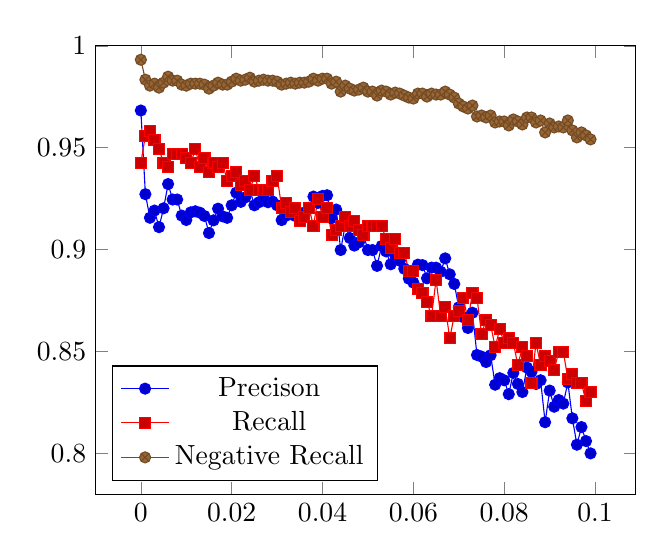
\begin{tikzpicture}
        \begin{axis}[
            legend pos=south west,
            ymax=1,
            xtick={0, 0.02, 0.04, 0.06, 0.08, 0.1},
            xticklabels={0, 0.02, 0.04, 0.06, 0.08, 0.1}
            ]
            \addplot+[sharp plot] coordinates {
            (0.000, 0.968254)
            (0.001, 0.927195)
            (0.002, 0.915612)
            (0.003, 0.919149)
            (0.004, 0.911017)
            (0.005, 0.920259)
            (0.006, 0.932166)
            (0.007, 0.924569)
            (0.008, 0.924569)
            (0.009, 0.916667)
            (0.010, 0.914530)
            (0.011, 0.918280)
            (0.012, 0.918803)
            (0.013, 0.918103)
            (0.014, 0.916488)
            (0.015, 0.908120)
            (0.016, 0.914347)
            (0.017, 0.920086)
            (0.018, 0.916309)
            (0.019, 0.915584)
            (0.020, 0.921739)
            (0.021, 0.927948)
            (0.022, 0.923414)
            (0.023, 0.925602)
            (0.024, 0.929360)
            (0.025, 0.921739)
            (0.026, 0.923246)
            (0.027, 0.925275)
            (0.028, 0.923246)
            (0.029, 0.923581)
            (0.030, 0.921739)
            (0.031, 0.914474)
            (0.032, 0.916667)
            (0.033, 0.918322)
            (0.034, 0.916484)
            (0.035, 0.917960)
            (0.036, 0.918142)
            (0.037, 0.920530)
            (0.038, 0.926009)
            (0.039, 0.922907)
            (0.040, 0.926339)
            (0.041, 0.926667)
            (0.042, 0.915367)
            (0.043, 0.919643)
            (0.044, 0.899782)
            (0.045, 0.912088)
            (0.046, 0.905702)
            (0.047, 0.901961)
            (0.048, 0.903509)
            (0.049, 0.907285)
            (0.050, 0.899782)
            (0.051, 0.899782)
            (0.052, 0.892009)
            (0.053, 0.901747)
            (0.054, 0.899123)
            (0.055, 0.892779)
            (0.056, 0.897155)
            (0.057, 0.894505)
            (0.058, 0.890591)
            (0.059, 0.885714)
            (0.060, 0.883772)
            (0.061, 0.892617)
            (0.062, 0.892377)
            (0.063, 0.885906)
            (0.064, 0.891156)
            (0.065, 0.891111)
            (0.066, 0.889140)
            (0.067, 0.895692)
            (0.068, 0.887872)
            (0.069, 0.883146)
            (0.070, 0.871681)
            (0.071, 0.866812)
            (0.072, 0.861538)
            (0.073, 0.868996)
            (0.074, 0.848291)
            (0.075, 0.847495)
            (0.076, 0.844828)
            (0.077, 0.848156)
            (0.078, 0.833693)
            (0.079, 0.836910)
            (0.080, 0.835853)
            (0.081, 0.829060)
            (0.082, 0.839479)
            (0.083, 0.834061)
            (0.084, 0.830108)
            (0.085, 0.842105)
            (0.086, 0.840000)
            (0.087, 0.834052)
            (0.088, 0.835886)
            (0.089, 0.815287)
            (0.090, 0.830803)
            (0.091, 0.822894)
            (0.092, 0.826180)
            (0.093, 0.824411)
            (0.094, 0.834802)
            (0.095, 0.817204)
            (0.096, 0.804255)
            (0.097, 0.812903)
            (0.098, 0.806034)
            (0.099, 0.800000)
            };
            \addlegendentry{Precison}
            \addplot+[sharp plot] coordinates {
            (0.000, 0.942605)
            (0.001, 0.955850)
            (0.002, 0.958057)
            (0.003, 0.953642)
            (0.004, 0.949227)
            (0.005, 0.942605)
            (0.006, 0.940397)
            (0.007, 0.947020)
            (0.008, 0.947020)
            (0.009, 0.947020)
            (0.010, 0.944812)
            (0.011, 0.942605)
            (0.012, 0.949227)
            (0.013, 0.940397)
            (0.014, 0.944812)
            (0.015, 0.938190)
            (0.016, 0.942605)
            (0.017, 0.940397)
            (0.018, 0.942605)
            (0.019, 0.933775)
            (0.020, 0.935982)
            (0.021, 0.938190)
            (0.022, 0.931567)
            (0.023, 0.933775)
            (0.024, 0.929360)
            (0.025, 0.935982)
            (0.026, 0.929360)
            (0.027, 0.929360)
            (0.028, 0.929360)
            (0.029, 0.933775)
            (0.030, 0.935982)
            (0.031, 0.920530)
            (0.032, 0.922737)
            (0.033, 0.918322)
            (0.034, 0.920530)
            (0.035, 0.913907)
            (0.036, 0.916115)
            (0.037, 0.920530)
            (0.038, 0.911700)
            (0.039, 0.924945)
            (0.040, 0.916115)
            (0.041, 0.920530)
            (0.042, 0.907285)
            (0.043, 0.909492)
            (0.044, 0.911700)
            (0.045, 0.916115)
            (0.046, 0.911700)
            (0.047, 0.913907)
            (0.048, 0.909492)
            (0.049, 0.907285)
            (0.050, 0.911700)
            (0.051, 0.911700)
            (0.052, 0.911700)
            (0.053, 0.911700)
            (0.054, 0.905077)
            (0.055, 0.900662)
            (0.056, 0.905077)
            (0.057, 0.898455)
            (0.058, 0.898455)
            (0.059, 0.889625)
            (0.060, 0.889625)
            (0.061, 0.880795)
            (0.062, 0.878587)
            (0.063, 0.874172)
            (0.064, 0.867550)
            (0.065, 0.885210)
            (0.066, 0.867550)
            (0.067, 0.871965)
            (0.068, 0.856512)
            (0.069, 0.867550)
            (0.070, 0.869757)
            (0.071, 0.876380)
            (0.072, 0.865342)
            (0.073, 0.878587)
            (0.074, 0.876380)
            (0.075, 0.858720)
            (0.076, 0.865342)
            (0.077, 0.863135)
            (0.078, 0.852097)
            (0.079, 0.860927)
            (0.080, 0.854305)
            (0.081, 0.856512)
            (0.082, 0.854305)
            (0.083, 0.843267)
            (0.084, 0.852097)
            (0.085, 0.847682)
            (0.086, 0.834437)
            (0.087, 0.854305)
            (0.088, 0.843267)
            (0.089, 0.847682)
            (0.090, 0.845475)
            (0.091, 0.841060)
            (0.092, 0.849890)
            (0.093, 0.849890)
            (0.094, 0.836645)
            (0.095, 0.838852)
            (0.096, 0.834437)
            (0.097, 0.834437)
            (0.098, 0.825607)
            (0.099, 0.830022)
            };
            \addlegendentry{Recall}
            \addplot+[sharp plot] coordinates {
            (0.000, 0.993161)
            (0.001, 0.983390)
            (0.002, 0.980459)
            (0.003, 0.981436)
            (0.004, 0.979482)
            (0.005, 0.981925)
            (0.006, 0.984856)
            (0.007, 0.982902)
            (0.008, 0.982902)
            (0.009, 0.980948)
            (0.010, 0.980459)
            (0.011, 0.981436)
            (0.012, 0.981436)
            (0.013, 0.981436)
            (0.014, 0.980948)
            (0.015, 0.978994)
            (0.016, 0.980459)
            (0.017, 0.981925)
            (0.018, 0.980948)
            (0.019, 0.980948)
            (0.020, 0.982413)
            (0.021, 0.983879)
            (0.022, 0.982902)
            (0.023, 0.983390)
            (0.024, 0.984367)
            (0.025, 0.982413)
            (0.026, 0.982902)
            (0.027, 0.983390)
            (0.028, 0.982902)
            (0.029, 0.982902)
            (0.030, 0.982413)
            (0.031, 0.980948)
            (0.032, 0.981436)
            (0.033, 0.981925)
            (0.034, 0.981436)
            (0.035, 0.981925)
            (0.036, 0.981925)
            (0.037, 0.982413)
            (0.038, 0.983879)
            (0.039, 0.982902)
            (0.040, 0.983879)
            (0.041, 0.983879)
            (0.042, 0.981436)
            (0.043, 0.982413)
            (0.044, 0.977528)
            (0.045, 0.980459)
            (0.046, 0.978994)
            (0.047, 0.978017)
            (0.048, 0.978505)
            (0.049, 0.979482)
            (0.050, 0.977528)
            (0.051, 0.977528)
            (0.052, 0.975574)
            (0.053, 0.978017)
            (0.054, 0.977528)
            (0.055, 0.976063)
            (0.056, 0.977040)
            (0.057, 0.976551)
            (0.058, 0.975574)
            (0.059, 0.974597)
            (0.060, 0.974108)
            (0.061, 0.976551)
            (0.062, 0.976551)
            (0.063, 0.975085)
            (0.064, 0.976551)
            (0.065, 0.976063)
            (0.066, 0.976063)
            (0.067, 0.977528)
            (0.068, 0.976063)
            (0.069, 0.974597)
            (0.070, 0.971666)
            (0.071, 0.970200)
            (0.072, 0.969223)
            (0.073, 0.970689)
            (0.074, 0.965315)
            (0.075, 0.965804)
            (0.076, 0.964827)
            (0.077, 0.965804)
            (0.078, 0.962384)
            (0.079, 0.962872)
            (0.080, 0.962872)
            (0.081, 0.960918)
            (0.082, 0.963850)
            (0.083, 0.962872)
            (0.084, 0.961407)
            (0.085, 0.964827)
            (0.086, 0.964827)
            (0.087, 0.962384)
            (0.088, 0.963361)
            (0.089, 0.957499)
            (0.090, 0.961895)
            (0.091, 0.959941)
            (0.092, 0.960430)
            (0.093, 0.959941)
            (0.094, 0.963361)
            (0.095, 0.958476)
            (0.096, 0.955056)
            (0.097, 0.957499)
            (0.098, 0.956033)
            (0.099, 0.954079)
            };
            \addlegendentry{Negative Recall}
            %\draw[red,line width=1pt] ({axis cs:0.002,0}|-{rel axis cs:0,1}) -- ({axis cs:0.002,0}|-{rel axis cs:0,0});
        \end{axis}
    \end{tikzpicture}
    \caption{Precision and recall w.r.t. lower threshold (no cap on the upper bound)}
    \label{p:lowerbound}
\end{figure}




